% LTeX: enabled=true

\subsection{Important Notation}

To avoid ambiguity, we introduce the following notation conventions used throughout the paper.
For any $n \in \mathbb{N}$, we write $[n] \triangleq \{1, \ldots, n\}$  and $[n]_0 \triangleq [n] \cup \{0\}$. 
We define the Boolean domain as $\mathbb{B} \triangleq \{0, 1\}$ and
three-value domain $\mathbb{T} \triangleq \{0, 1, \bot\}$.


\subsection{Background overview}


\subsubsection{Counting Complexity and Combinatorial Interpretations}

The general idea of combinatorial interpretations is, given a function $f: \mathbb{B}^n \to \mathbb{N}$, 
for every word $w$, we want to find a set $A_w$ such that $f(w)= |A_w|$.
To ground that notion, researchers looked into counting complexity.
In the current project we will focus specifically on the $\textsc{\#P}$ class.
$\textsc{\#P}$ was introduced by Valiant \cite{valiant_ComplexityComputingPermanent_1979},
to demonstrate the difficulty of counting the number of solutions to a problem,
where each solution can be verified in polynomial time, or more formally:

\begin{definitionbox}{$\textsc{\#P}$ Complexity Clas \cite{valiant_ComplexityComputingPermanent_1979}}{sharpp-class}
    A function $f: \mathbb{B}^* \to \mathbb{N} \in \textsc{\#P}$, if there exists a
    poly-function $p : \mathbb{N} \to \mathbb{N}$ and a poly-time TM $M$ such that:
    $$
    f(w) = \Big|\Big\{v \in \mathbb{B}^{p(|w|)} \mid M(w, v) =1 \Big\}\Big|
    $$
\end{definitionbox}

Given the above definition, Pak et al. \cite{pak_WhatCombinatorialInterpretation_2022, ikenmeyer_PositivitySymmetricGroup_2024}
used $\textsc{\#P}$ to interpret $A_w$ as the set of solutions to a problem given input $w$.
Moreover, they argue that the usage of $\textsc{\#P}$ has several benefits:

\begin{enumerate}
    \item By polynomially bounding words, we avoid cases such as: $f(w) = |\{1, \hdots, f(w)\}|$.
    \item We can work with $f(\cdot)$, even if its direct computation is hard.
    \item $\textsc{\#P}$ is a formal system that is highly flexible.
\end{enumerate}

The current framework was used in several papers such as
\cite{ikenmeyer_WhatWhatNot_2022} and \cite{ikenmeyer_PositivitySymmetricGroup_2024}
to demonstrate the existence of combinatorial interpretations.
Lastly, we introduce the idea of correlating two counting problems with the help of
\textit{parsimonious reductions} \ref{def:pars-reduction}.


\begin{definitionbox}{Parsimonious reductions}{pars-reduction}
    Let $R, R'$ be search problems, and let $f$ be a reduction of
    $S_R = \{x \mid R(x) \neq \emptyset \}$ to $S_{R'} = \{x \mid R'(x) \neq \emptyset \}$.
    We say $f$ is \textbf{parsimonious} if:
    $$
    \forall x \in S_R : |R(x)| = |R'(f(x))|
    $$ 
\end{definitionbox}

The definition below introduces a variant of parsimonious reductions that allows
for one-to-many reductions. 
\begin{definitionbox}{Poly-Function Bounded Parsimonious Reductions}{func-pars}
    Given two counting problems $A, B : \mathbb{B}^* \to \mathbb{N}$
    and a poly-function $f : \mathbb{N} \to \mathbb{N}$, we
    say that:
    $$
    A \subseteq^f B \iff \forall x \in \mathbb{B}^n:  A(x) \leq B(x) \leq f(|x|) \cdot A(x)
    $$
    If $\forall x : f(x) = c$ for $c \in \mathbb{N}$, we use the abbreviation:
    $$
    A \subseteq^c B
    $$
\end{definitionbox}

\subsubsection{Total Search Problems and PPAD}
We give a brief overview of total search problems and their relevancy with the project.

\begin{definitionbox}{Search Problems and Total Search Problems}{search-problems}
    \textbf{Search problems} can be defined as relations $R \subseteq \mathbb{B}^* \times \mathbb{B}^*$,
    where given $x \in \mathbb{B}^*$, we want to find $y \in \mathbb{B}^*$  such that $xRy$.

    \textbf{Total Search problems} are search problems such that for each input, there must exist at least one solution.
\end{definitionbox}


\begin{definitionbox}{$\scn{FNP}$ and $\scn{TFNP}$}{fnp-tfnp}
    \textbf{FNP} are \textit{search problems} such that there exists poly-time TM $M: \mathbb{B}^* \to \mathbb{B}$
    and a poly function $p : \mathbb{N} \to \mathbb{N}$ such that:
    $$
    \forall x \in \mathbb{B}^*, y \in \mathbb{B}^{p(|x|)}: xRy \iff M(x,y) = 1
    $$
    Lastly $\textbf{TFNP} = \{L \in \textbf{FNP} \mid L \text{ is total}\}$
\end{definitionbox}
 

\begin{minipage}{0.55\linewidth}
\begin{definitionbox}{\textit{EndOfLine} problem \cite{papadimitriou_ComplexityParityArgument_1994}}{eol-ppad}
    Given poly-sized circuits $S, P \in \mathbb{B}^n \to \mathbb{B}^n$,
    we define a digraph $G = (V,E)$, such that $V= \mathbb{B}^n$ and $E$ defined as:
    $$
    E = \{(x,y) \in V^2: S(x) = y \wedge P(y) = x\}
    $$
    We define source nodes as $v \in V: \textit{deg}(v) = (0,1)$  and sink nodes as
    $\textit{deg}(v) = (1,0)$. 
    We also syntactically ensure that the $0^n$ node is always a source, meaning
    $S(P(0^n)) \neq 0 \wedge P(S(0^n)) = 0^n$.
    A node $v \in V$ is a solution \textit{iff} $\textit{in-deg}(v) \neq \textit{out-deg}(v)$.
\end{definitionbox}
\end{minipage}
\begin{minipage}{0.45\linewidth}
    \centering
    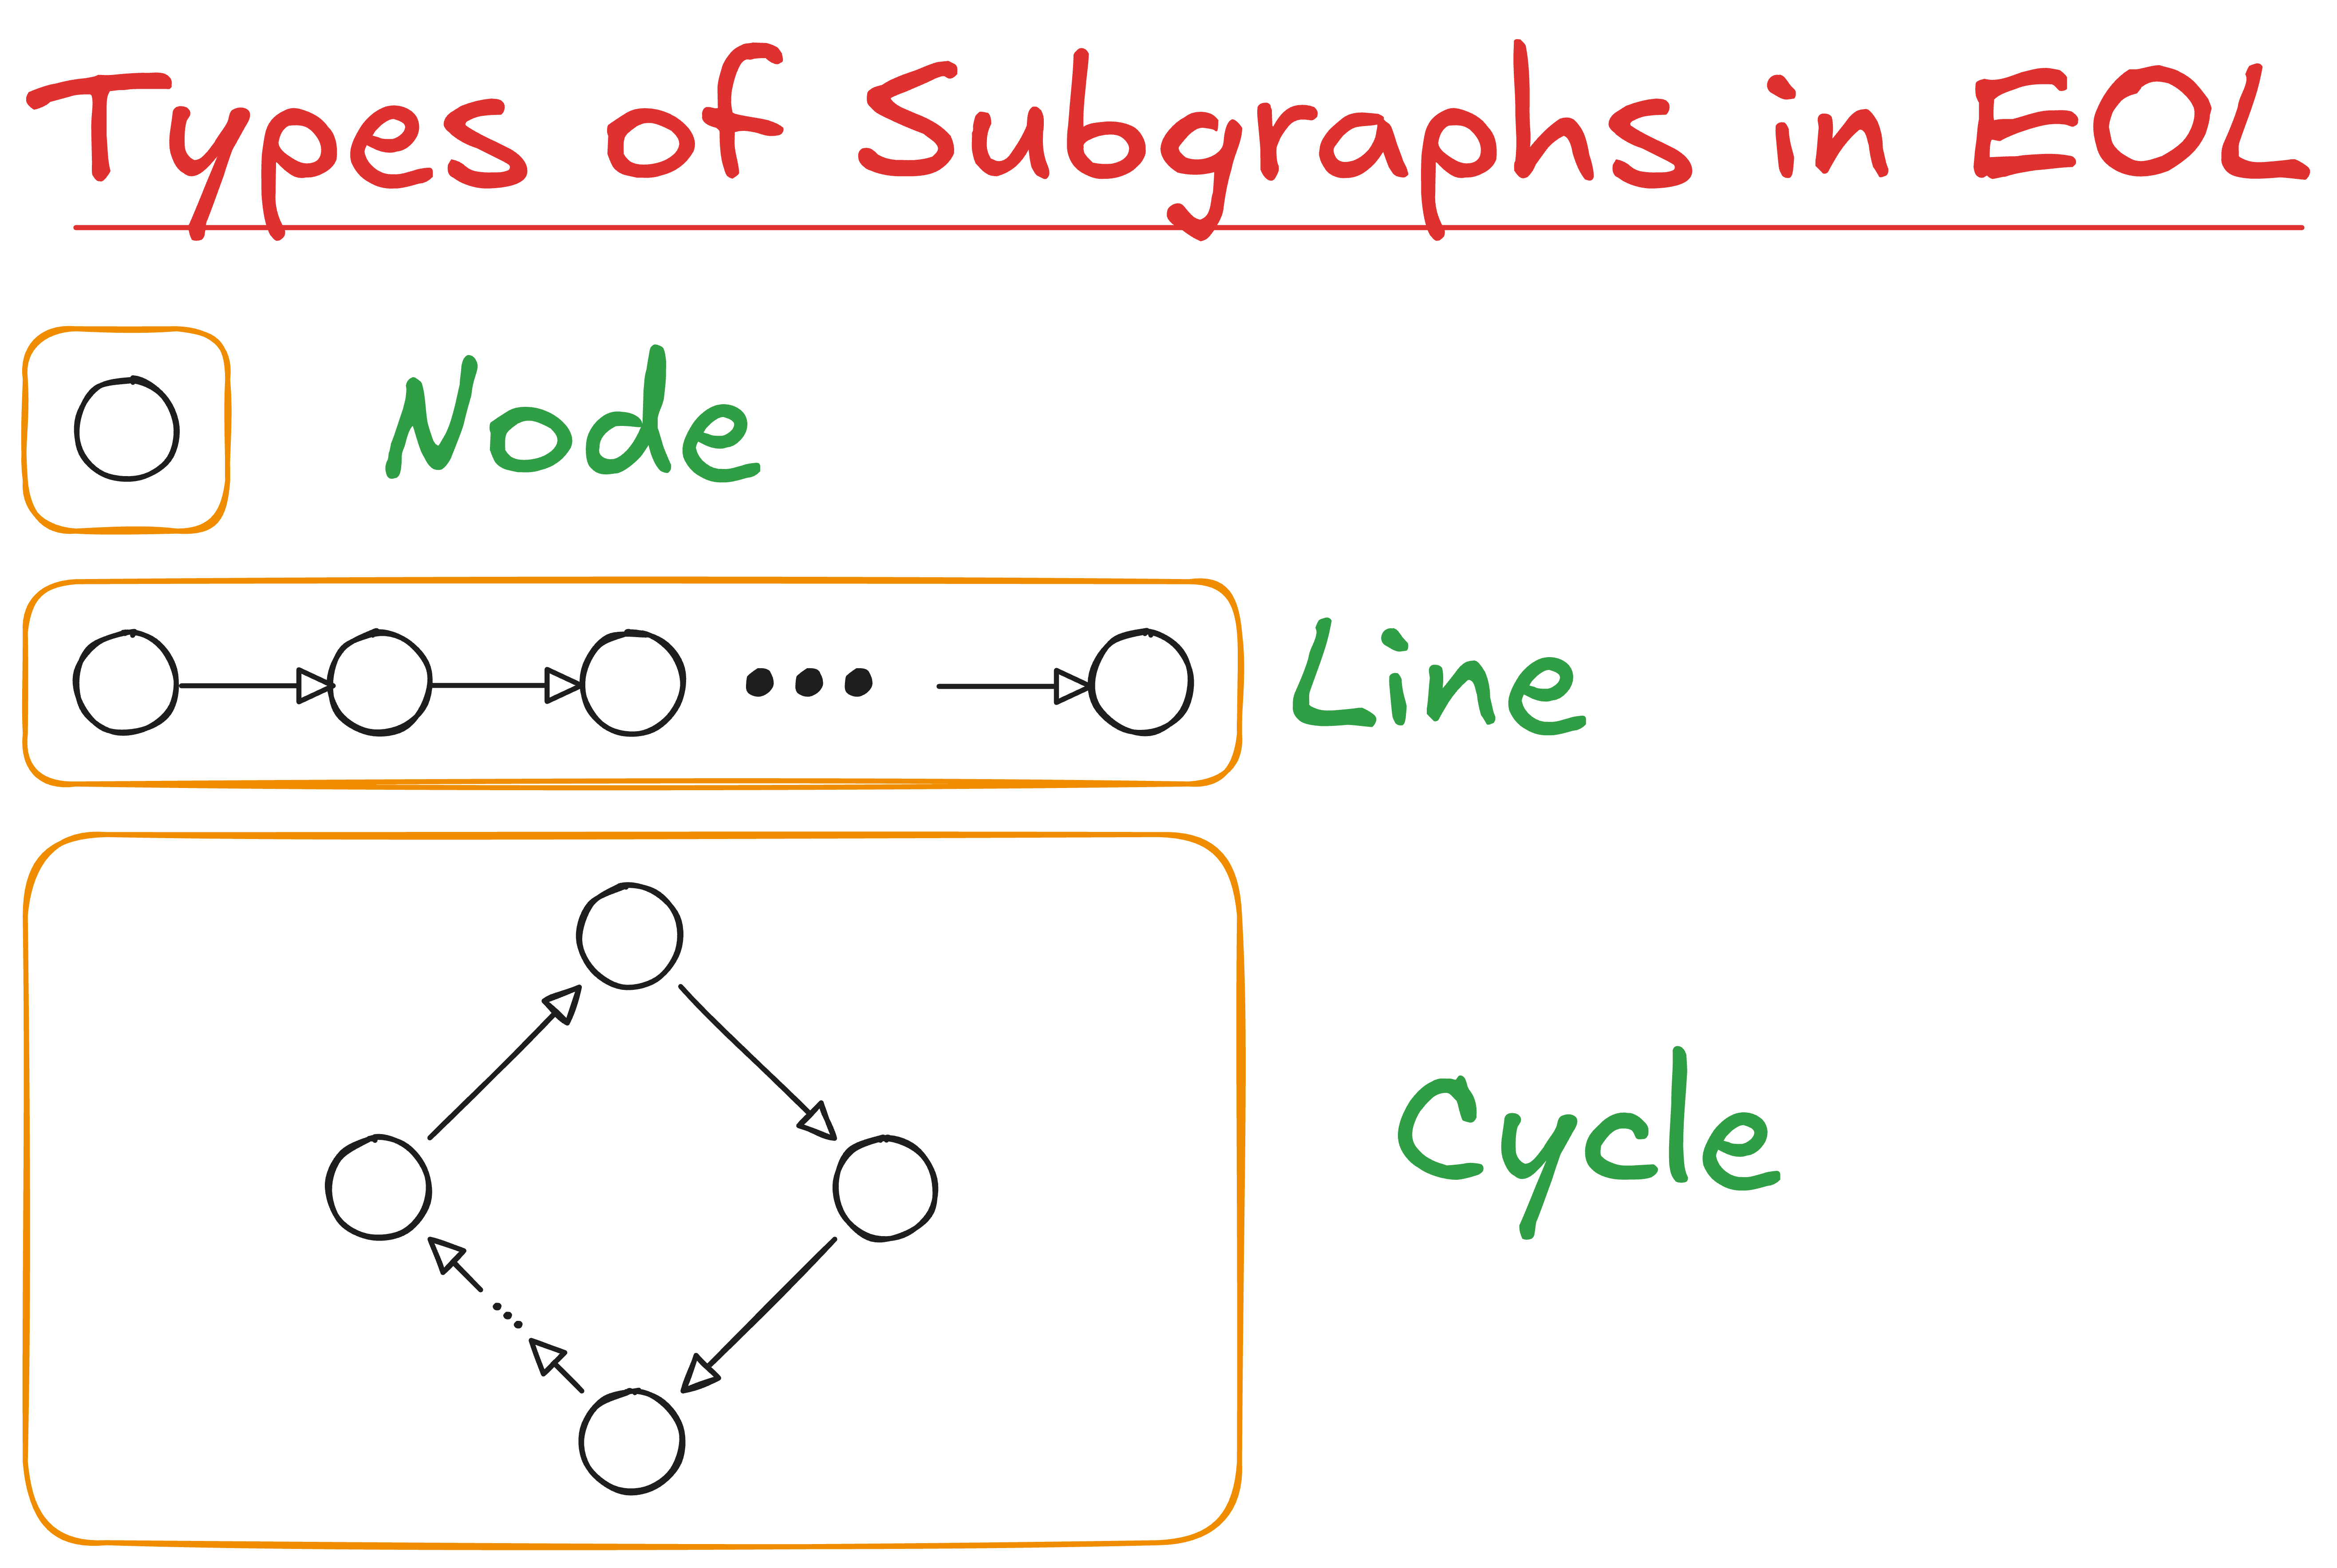
\includegraphics[width=0.7\linewidth]{assets/eol-subgraphs.png}
    \captionof{figure}{Types of subgraphs in \textsc{EndOfLine}}\label{fig:eol-subgraphs}
\end{minipage}

\vspace{0.2cm}

An illustrative example of an \textsc{EndOfLine} instance can be seen in figure \ref{fig:eol-subgraphs}. 
From this problem, we define the \textsc{PPAD} complexity class \ref{def:ppad-complexity-class}.


\begin{definitionbox}{\textsc{PPAD} complexity class \cite{papadimitriou_ComplexityParityArgument_1994}}{ppad-complexity-class}
    \textsc{PPAD} is defined as the set of search problems that
    are reducible to the \scn{EndOfLine} problem \ref{def:eol-ppad}.
\end{definitionbox}

\textsc{PPAD} has been created by Papadimitriou \cite{papadimitriou_ComplexityParityArgument_1994}
to demonstrate a subset of problems in \textsc{NP} that guarantee
a solution but believed to be very inefficient to find.
In the next section,
we introduce relevant \textsc{PPAD} problems.

\paragraph{The PureCircuit problem}
\label{par:pure-circ-def}

The definition of \textsc{PureCircuit} is based Kleene's three-valued strong logic of indeterminacy,
which extends the traditional binary logic \cite{kleene_IntroductionMetamathematics_2009}.
This problem was created by Deligkas et al. \cite{deligkas_PureCircuitTightInapproximability_2024}
to demonstrate the hardness of approximating \textsc{PPAD} problems and was shown to be \textsc{PPAD-complete}.


\begin{definitionbox}{\textsc{PureCiruit} Problem Definition \cite{deligkas_PureCircuitTightInapproximability_2024}}{purecircuit-def}
An instance of \textit{PureCircuit} is given by vertex set $V= [n]$ and gate set $G$ such that
$\forall g \in G: g=(T,u,v,w)$ where $u,v,w \in V$ and $T \in \{\text{NOR}, \text{Purify}\}$.
Each gate is interpreted as:
\begin{enumerate}
    \item \textit{NOR}: Takes as input $u,v$ and outputs $w$
    \item \textit{Purify}: Takes as input $u$ and outputs $v,w$
\end{enumerate}
And each vertex is ensured to have $\text{in-deg}(v) \leq 1$.
A solution to input instance $(V,G)$ is denoted as an assignment $\mathbf{x} : V \to \{0, \bot, 1\}$
such that for all gates $g = (T,u,v,w)$ we have:
\begin{enumerate}
    \item \textit{NOR}:
       \begin{gather*}
            \mathbf{x}[u] = \mathbf{x}[v] = 0 \implies \mathbf{x}[w] = 1\\
            (\mathbf{x}[u] =1 \vee \mathbf{x}[v] =1) \implies \mathbf{x}[w] = 0 \\
            \text{otherwise} \implies \bot
        \end{gather*}

    \item \textit{Purify}: 
       \begin{gather*}
           \forall b \in \mathbb{B}: \mathbf{x}[u] = b \implies \mathbf{x}[v] = b \wedge \mathbf{x}[w] =  b\\
           \mathbf{x}[u] = \bot \implies \{\mathbf{x}[v] \cup \mathbf{x}[w] \} \cap \mathbb{B}\neq \emptyset
        \end{gather*}
\end{enumerate}
\end{definitionbox}

In addition to the gates above, we will make use of the standard set of gates $\{\vee, \wedge, \neg\}$,
whose behaviour is depicted in the tables \ref{tab:three-val-logic}.
Moreover, we will make use of the \textit{Copy} gate which we can define as $\textit{Copy}(x) = \neg (\neg x)$.
These gates are well defined based on the \textit{NOR} gate as shown by Deligkas et al. \cite{deligkas_PureCircuitTightInapproximability_2024}
and do not directly affect the complexity of the problem.
Furthermore, with respect to the \textit{Purify} gate,
Deligkas et al. \cite{deligkas_PureCircuitTightInapproximability_2024} showed that the only \textit{Purify} solutions essential
for \textsc{PPAD-completeness} are $\{(0,\bot), (\bot,1), (0,1)\}$, and the addition of more solutions does not affect its complexity.
We will base our constructions around that limited set of solutions.
We acknowledge that this simplified variant of the problem captures a subset of the original set of solutions, but
one can observe that $\textsc{\#PureCircuit-simplified} \subseteq \textsc{\#PureCircuit}$,
and therefore any proposition or argument of the sort:
$\textsc{\#A} \subseteq \textsc{\#PureCircuit-simplified} \implies \textsc{\#A} \subseteq \textsc{\#PureCircuit}$.
All solution sets will be made explicit before analysing the counting complexity of the problem,
and we will refer to all such simplified variants as $\textsc{\#PureCircuit}$ as they do not impact 
the overall reduction. 

\begin{table}[h!]
    \centering
    \subfloat[\texttt{not} gate]{
    \begin{tabular}{c|c}
\texttt{not} & \textbf{} \\
\hline
0 & 1 \\
$\bot$ & $\bot$ \\
1 & 0 \\
\end{tabular}
}
\subfloat[\texttt{and} gate]{
\begin{tabular}{c|ccc}
\texttt{and} & 0 & $\bot$ & 1 \\
\hline
0    & 0 & 0 & 0 \\
$\bot$ & 0 & $\bot$ & $\bot$ \\
1    & 0 & $\bot$ & 1 \\
\end{tabular}
} \quad
\subfloat[\texttt{or} gate]{
\begin{tabular}{c|ccc}
\texttt{or} & 0 & $\bot$ & 1 \\
\hline
0    & 0     & $\bot$ & 1 \\
$\bot$ & $\bot$  & $\bot$ & 1 \\
1    & 1 & 1 & 1 \\
\end{tabular}
}

    \caption{Three-valued logic \cite{kleene_IntroductionMetamathematics_2009}}\label{tab:three-val-logic}
\end{table}

%
% \begin{definitionbox}{\textsc{SourceOrExcess} problem \cite{ikenmeyer_WhatWhatNot_2022}}{source-or-excess}
%     We define as $\textit{SourceOrExcess}(k,1)$ for $k \in \mathbb{N}_{\geq 2}$
%     the search problem as such: Given a poly-sized successor circuit $S : \mathbb{B}^n$
%     and a set of predecessor poly-sized circuits $\{P_i\}_{i \in [k]}$, we define
%     the graph $G = (V,E)$ such that, $V = \mathbb{B}^n$ and $E$ as:
%     $$
%     \forall x, y \in V: (x,y) \in E \iff (S(x) = y) \wedge \bigvee_{i \in [k]} P_i(y) = x
%     $$
%     We ensure that $0^n$ is as source, meaning $\text{deg}(0^n) = (0,1)$.
%     A valid solution is a vertex $v$ such that $\textit{in-deg}(v) \neq \textit{out-deg}(v)$
% \end{definitionbox}
%
% The above problem generalises the \textsc{EndOfLine} problem which 
% does not have an explicit combinatorial interpretation as Ikenmeyer et al. \cite{ikenmeyer_WhatWhatNot_2022}
% demonstrated.

\paragraph{Sperner problems}

Below we will refer to the notion of Sperner problems, which uses
the topology of a problem and a colouring scheme to ensure
that a substructure is panchromatic. There are two variants of colouring scheme
that are used: the first will be referred to as the \textbf{linear} colouring
where for dimension $d$, assign $d+1$ distinct colours to each point \cite{daskalakis_ComplexityComputingNash_2006, chen_Complexity2DDiscrete_2009}.
Subsequently, we will refer to \textbf{bipolar} colouring, which has been used in grid-like topologies of the Sperner property
\cite{chen_SettlingComplexityComputing_2009, deligkas_PureCircuitTightInapproximability_2024, daskalakis_ComplexityConstrainedMinmax_2021}.
We note that these terms are not standard in literature; we adopt this naming convention
for of clarity.



\begin{definitionbox}{Bipolar colouring}{bipolar-colouring}
    Given a set $S^d$, where $S$ is some arbitrary set, we refer
    to bipolar colouring $C$ as:
    $$
    \forall v \in S^d, j \in [d]: [C(v)]_j \in \{-1,1\}
    $$
    We say that a set of points $A \subseteq S^d$ \textbf{cover all the labels} if:
    $$
        \forall i \in [d], \ell \in \{-1, +1\}, \exists x \in A: [\lambda(x)]_{i} = \ell
    $$

\end{definitionbox}

Deligkas et al. \cite{deligkas_PureCircuitTightInapproximability_2024, deligkas_ConstantInapproximabilityPPA_2022} showed that
$\forall A \subseteq S^d: |A| \geq d+1$ and satisfies the colouring, $\exists D \subseteq A: |D| \leq d$ where $D$ also satisfies
the colouring condition.

\begin{definitionbox}{\textsc{StrongSperner} problem}{strong-sperner}
    \textbf{Input}: A boolean circuit that computes a bipolar labelling $\lambda: [M]^N \to \{-1, 1\}^N$ \ref{def:bipolar-colouring}
    satisfying the following boundary conditions for every $i \in [N]$:
    \begin{itemize}
        \item if $x_i = 1 \implies [\lambda(x)]_i = +1$
        \item if $x_i = M \implies [\lambda(x)]_i = -1$
    \end{itemize}
    \textbf{Output}: A set of points $\{x^{(i)}\}_{i \in [N]} \subseteq [M]^{N}$, such that:
    \begin{itemize}
        \item \textit{Closeness condition}: $\forall i,j \in [N]: \|x^{(i)} - x^{(j)}\|_{\infty} \leq 1$
        \item \textit{Covers all labels} as defined in \ref{def:bipolar-colouring}
    \end{itemize}
\end{definitionbox}

The above is a generalised variant of the traditional Sperner problem to
a grid of dimensions $N$ with width of $M$. 
Throughout literature the same variants of the problem or specifications
have been defined using the names Sperner or discrete Brouwer \cite{chen_SettlingComplexityComputing_2009, chen_Complexity2DDiscrete_2009, daskalakis_ComplexityComputingNash_2006, deligkas_PureCircuitTightInapproximability_2024}.
For clarity, the subsequent analysis adopts $\textsc{StrongSperner}$.

\begin{definitionbox}{$\scn{nD-StrongSperner}$ problem}{nd-strong-sperner}
    \textbf{Input}: A tuple $(\lambda,0^k)$ of a $\scn{StrongSperner}$ instance but for only $n$ dimensions, such that
    $\lambda : (\mathbb{B}^k)^n \to \{-1, +1\}^n$.\\
    \textbf{Output}: A point $\alpha = (a_1, \hdots, a_n) \in (\mathbb{B}^k \setminus \{1^k\})^n$ such that
    $$
    \{\alpha + x \mid x \in \mathbb{B}^n\} \text{ covers all the labels \ref{def:bipolar-colouring}}
    $$
    We assume dimensionality $n \geq 2$.
\end{definitionbox}

The authors refer to both colouring schemes interchangeably when discussing their reductions,
so we can assume that all reductions (not necessarily counting reductions) work similarly for either colouring
\cite{chen_SettlingComplexityComputing_2009, deligkas_PureCircuitTightInapproximability_2024, daskalakis_ComplexityComputingNash_2006, chen_Complexity2DDiscrete_2009}.


\paragraph{Other PPAD problems} 

We will define several problems in \textsc{PPAD} that are related with our project
and demonstrate the counting complexity of \textsc{PureCircuit}.

\begin{definitionbox}{\textsc{SourceOrExcess} problem \cite{ikenmeyer_WhatWhatNot_2022}}{source-or-excess}
    We define as $\textsc{SourceOrExcess(k,1)}$ for $k \in \mathbb{N}_{\geq 2}$
    the search problem as such: Given a poly-sized successor circuit $S : \mathbb{B}^n \to \mathbb{B}^n$
    and a set of predecessor poly-sized circuits $\{P_i\}_{i \in [k]}$, where $P_i : \mathbb{B}^n \to \mathbb{B}^n$, we define
    the graph $G = (V,E)$ such that, $V = \mathbb{B}^n$ and $E$ as:
    $$
    \forall x, y \in V: (x,y) \in E \iff (S(x) = y) \wedge \bigvee_{i \in [k]} P_i(y) = x
    $$
    We ensure that $0^n$ is as sink, meaning $\text{deg}(0^n) = (0,1)$.
    A valid solution is a vertex $v$ such that $\textit{in-deg}(v) \neq \textit{out-deg}(v)$
\end{definitionbox}

The $\textsc{SourceOrExcess(k,1)}$ problem can be considered as the generalisation of the \textsc{EndOfLine}
problem for graphs with $\textit{in-deg}(\cdot) \leq k$ and $\textit{out-deg}(\cdot) \leq 1$.
Lastly, we will introduce \textsc{Tarski} \ref{def:tarski-ppad}
which uses the Knaster-Tarski fixed point theorem \ref{thm:knaster-tarski} and
belongs in $\textsc{PLS} \cap \textsc{PPAD}$,
where  $\textsc{PLS}$ is a class of problems based on the idea of local search \cite{johnson_HowEasyLocal_1988}.
%
%
\begin{definitionbox}{Monotone functions}{mono-func}
    Given two partially ordered sets $(L_1, \preceq_{L_1})$ and $(L_2, \preceq_{L_2})$, a function
    $f: L_1 \to L_2$ is \textbf{monotone} if and only if:
    $$
    \forall x,y \in L_1: x \preceq_{L_1} y \implies f(x) \preceq_{L_2} f(y)
    $$
\end{definitionbox}
%     
%
\begin{theorembox}{Knaster Tarski Fixed point theorem\cite{bronislaw_TheoremeFunctionsDensembles_1928, fearnley_FasterAlgorithmFinding_2022}}{knaster-tarski}
    Given a \textit{monotone} function $f: L \to L$ \ref{def:mono-func} of a complete lattice $(L, \wedge, \vee)$,  $\exists c \in L: f(c) = c$.
\end{theorembox}

\begin{definitionbox}{$\scn{Tarski}$ problem definition \cite{fearnley_FasterAlgorithmFinding_2022}}{tarski-ppad}
    Given a \textit{monotone} function $f: L \to L$ \ref{def:mono-func} of a lattice $(L, \wedge, \vee)$
    we define solutions to the problem as:
    \begin{enumerate}
        \item Find $x \in L: f(x) = x$
        \item Find $x,y \in L$ such that $x \preceq y$ and $f(x) \not\preceq f(y)$
    \end{enumerate}
    We assume that $f$ is represented by boolean circuits.
\end{definitionbox}
%
\paragraph{Counting complexity of PPAD}
\label{par:count-ppad}


Ikenmeyer et al. \cite{ikenmeyer_WhatWhatNot_2022} demonstrated that several \textsc{PPAD-complete}
problems behave differently under $\textsc{\#PPAD} -1$. More specifically
$\textsc{\#EndOfLine} - 1 \subseteq \textsc{\#P}$ but $\exists A: \textsc{\#SourceOrExcess}^A  - 1\not\subseteq \textsc{\#P}^A$.
We estimate the counting difficulty of the aforementioned problems based on their position in the hierarchy as seen in the figure \ref{fig:ppad-count-hier}.

\begin{figure}[h!]
    \centering
    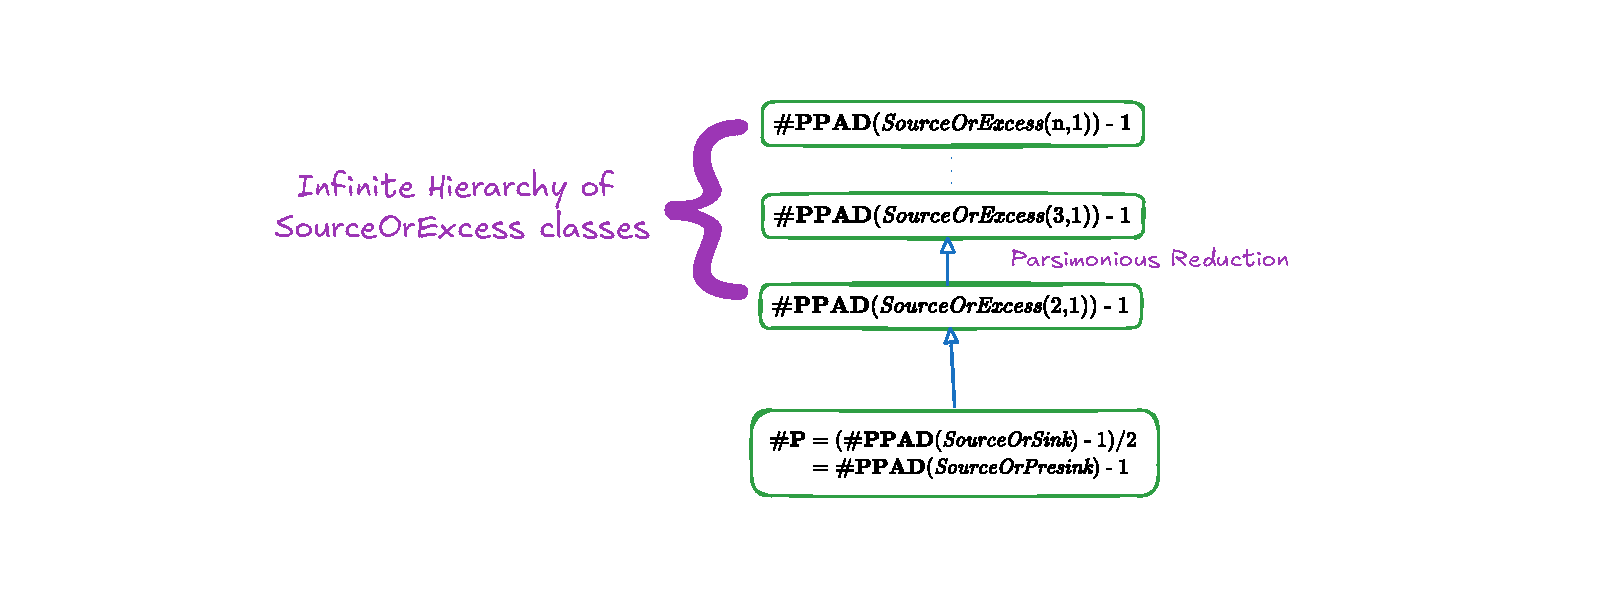
\includegraphics[width=0.75\textwidth]{assets/chart-plot.pdf}
    \caption{Counting hierarchy graph between \textsc{\#PPAD-complete} problems. Figure obtained from \cite{ikenmeyer_WhatWhatNot_2022}.}\label{fig:ppad-count-hier}
\end{figure}


\subsubsection{Kleene Logic and Hazard-Free Circuits}

Kleene logic uses the boolean system with an additional \textit{unstable} value \cite{kleene_IntroductionMetamathematics_2009}. 
The study of Kleene logic assisted in
the development of robust physical systems \cite{friedrichs_MetastabilityContainingCircuits_2018}, in addition to defining frameworks like \textit{Alternative Turing machines} \cite{kozen_TheoryComputation_2006}, and
aiding in the development of lower bounds for monotone circuits
\cite{eichelberger_HazardDetectionCombinational_1965, ikenmeyer_ComplexityHazardfreeCircuits_2019,ikenmeyer_KarchmerWigdersonGamesHazardfree_2022,  bund_SmallHazardFreeTransducers_2025}. 
The current section offers a brief summary to relevant notions and concepts in Kleene logic.

\begin{definitionbox}{Kleene value ordering \cite{mukaidono_BternaryLogicFunction_1972}}{kleene-order}
    The instability ordering for $\leq^u$ is defined as: $\bot \leq^u 0,1$. The $n$-dimensional
    extension of the ordering is:
    $$
    \forall x,y \in \mathbb{T}^n: x \leq^u y \implies \forall j \in [n]: (x_j \in \mathbb{B} \implies x_i = y_i)
    $$
\end{definitionbox}


\begin{definitionbox}{Kleene Resolutions \cite{mukaidono_BternaryLogicFunction_1972, ikenmeyer_ComplexityHazardfreeCircuits_2019}}{kleene-res}
    Given $x \in \mathbb{T}^n$, we define the \textit{resolutions} of $x$, using the following notation:
    $$
    \scn{Res}(x) \triangleq \big\{ y \in \mathbb{B}^n \mid x \leq^u y  \big\}
    $$
\end{definitionbox}

Unless otherwise specified, we assume that all Kleene functions are \textit{natural} \ref{def:nat-func}, since
they can be represented by circuits \ref{prop:nat-func-circ}.
Detecting hazards is a concept that is analysed heavily when talking about Kleene logic.
The idea is ensuring robustness in our circuits, meaning if all resolutions of $x \in \mathbb{T}^n$
give the same value, then we should expect the circuit to behave the same way \ref{def:hf-def}.
An example of hazard values can be seen in the figure \ref{fig:hazard-example}.


\begin{definitionbox}{Natural functions \cite{ikenmeyer_ComplexityHazardfreeCircuits_2019}}{nat-func}
    A function $F: \mathbb{T}^n \to \mathbb{T}^m$ for some $n, m \in \mathbb{N}$ is \textit{natural} if and only
    if it satisfies the following properties:
    \begin{enumerate}
        \item \textit{Preserves stable values}: $\forall x \in \mathbb{B}^n: F(x) \in \mathbb{B}^m$ 
    \item \textit{Preserves monotonicity} \ref{def:mono-func} \ref{def:kleene-res}
    \end{enumerate}
\end{definitionbox}

\begin{propositionbox}{Natural functions and Circuits \cite{mukaidono_BternaryLogicFunction_1972,ikenmeyer_ComplexityHazardfreeCircuits_2019}}{nat-func-circ}
    A function $F: \mathbb{T}^n \to \mathbb{T}^m$ can be computed by a circuit \textit{iff} $F$ is \textit{natural} \ref{def:nat-func}
\end{propositionbox}

\begin{definitionbox}{Hazard \cite{ikenmeyer_ComplexityHazardfreeCircuits_2019, eichelberger_HazardDetectionCombinational_1965}}{hf-def}
    A \textit{circuit} $C$, on $n$ inputs has \textbf{hazard} at $x \in \mathbb{T}^n \iff C(x) = \bot$
    and $\exists b \in \mathbb{B}, \forall r \in \scn{Res}(x): C(r) = b$. If such value does not exists
    then we say that $C$ is hazard-free.
\end{definitionbox}

\begin{figure}[h!]
    \centering
    \subfloat[Multiplexer with hazard at $(1,1,\bot)$]{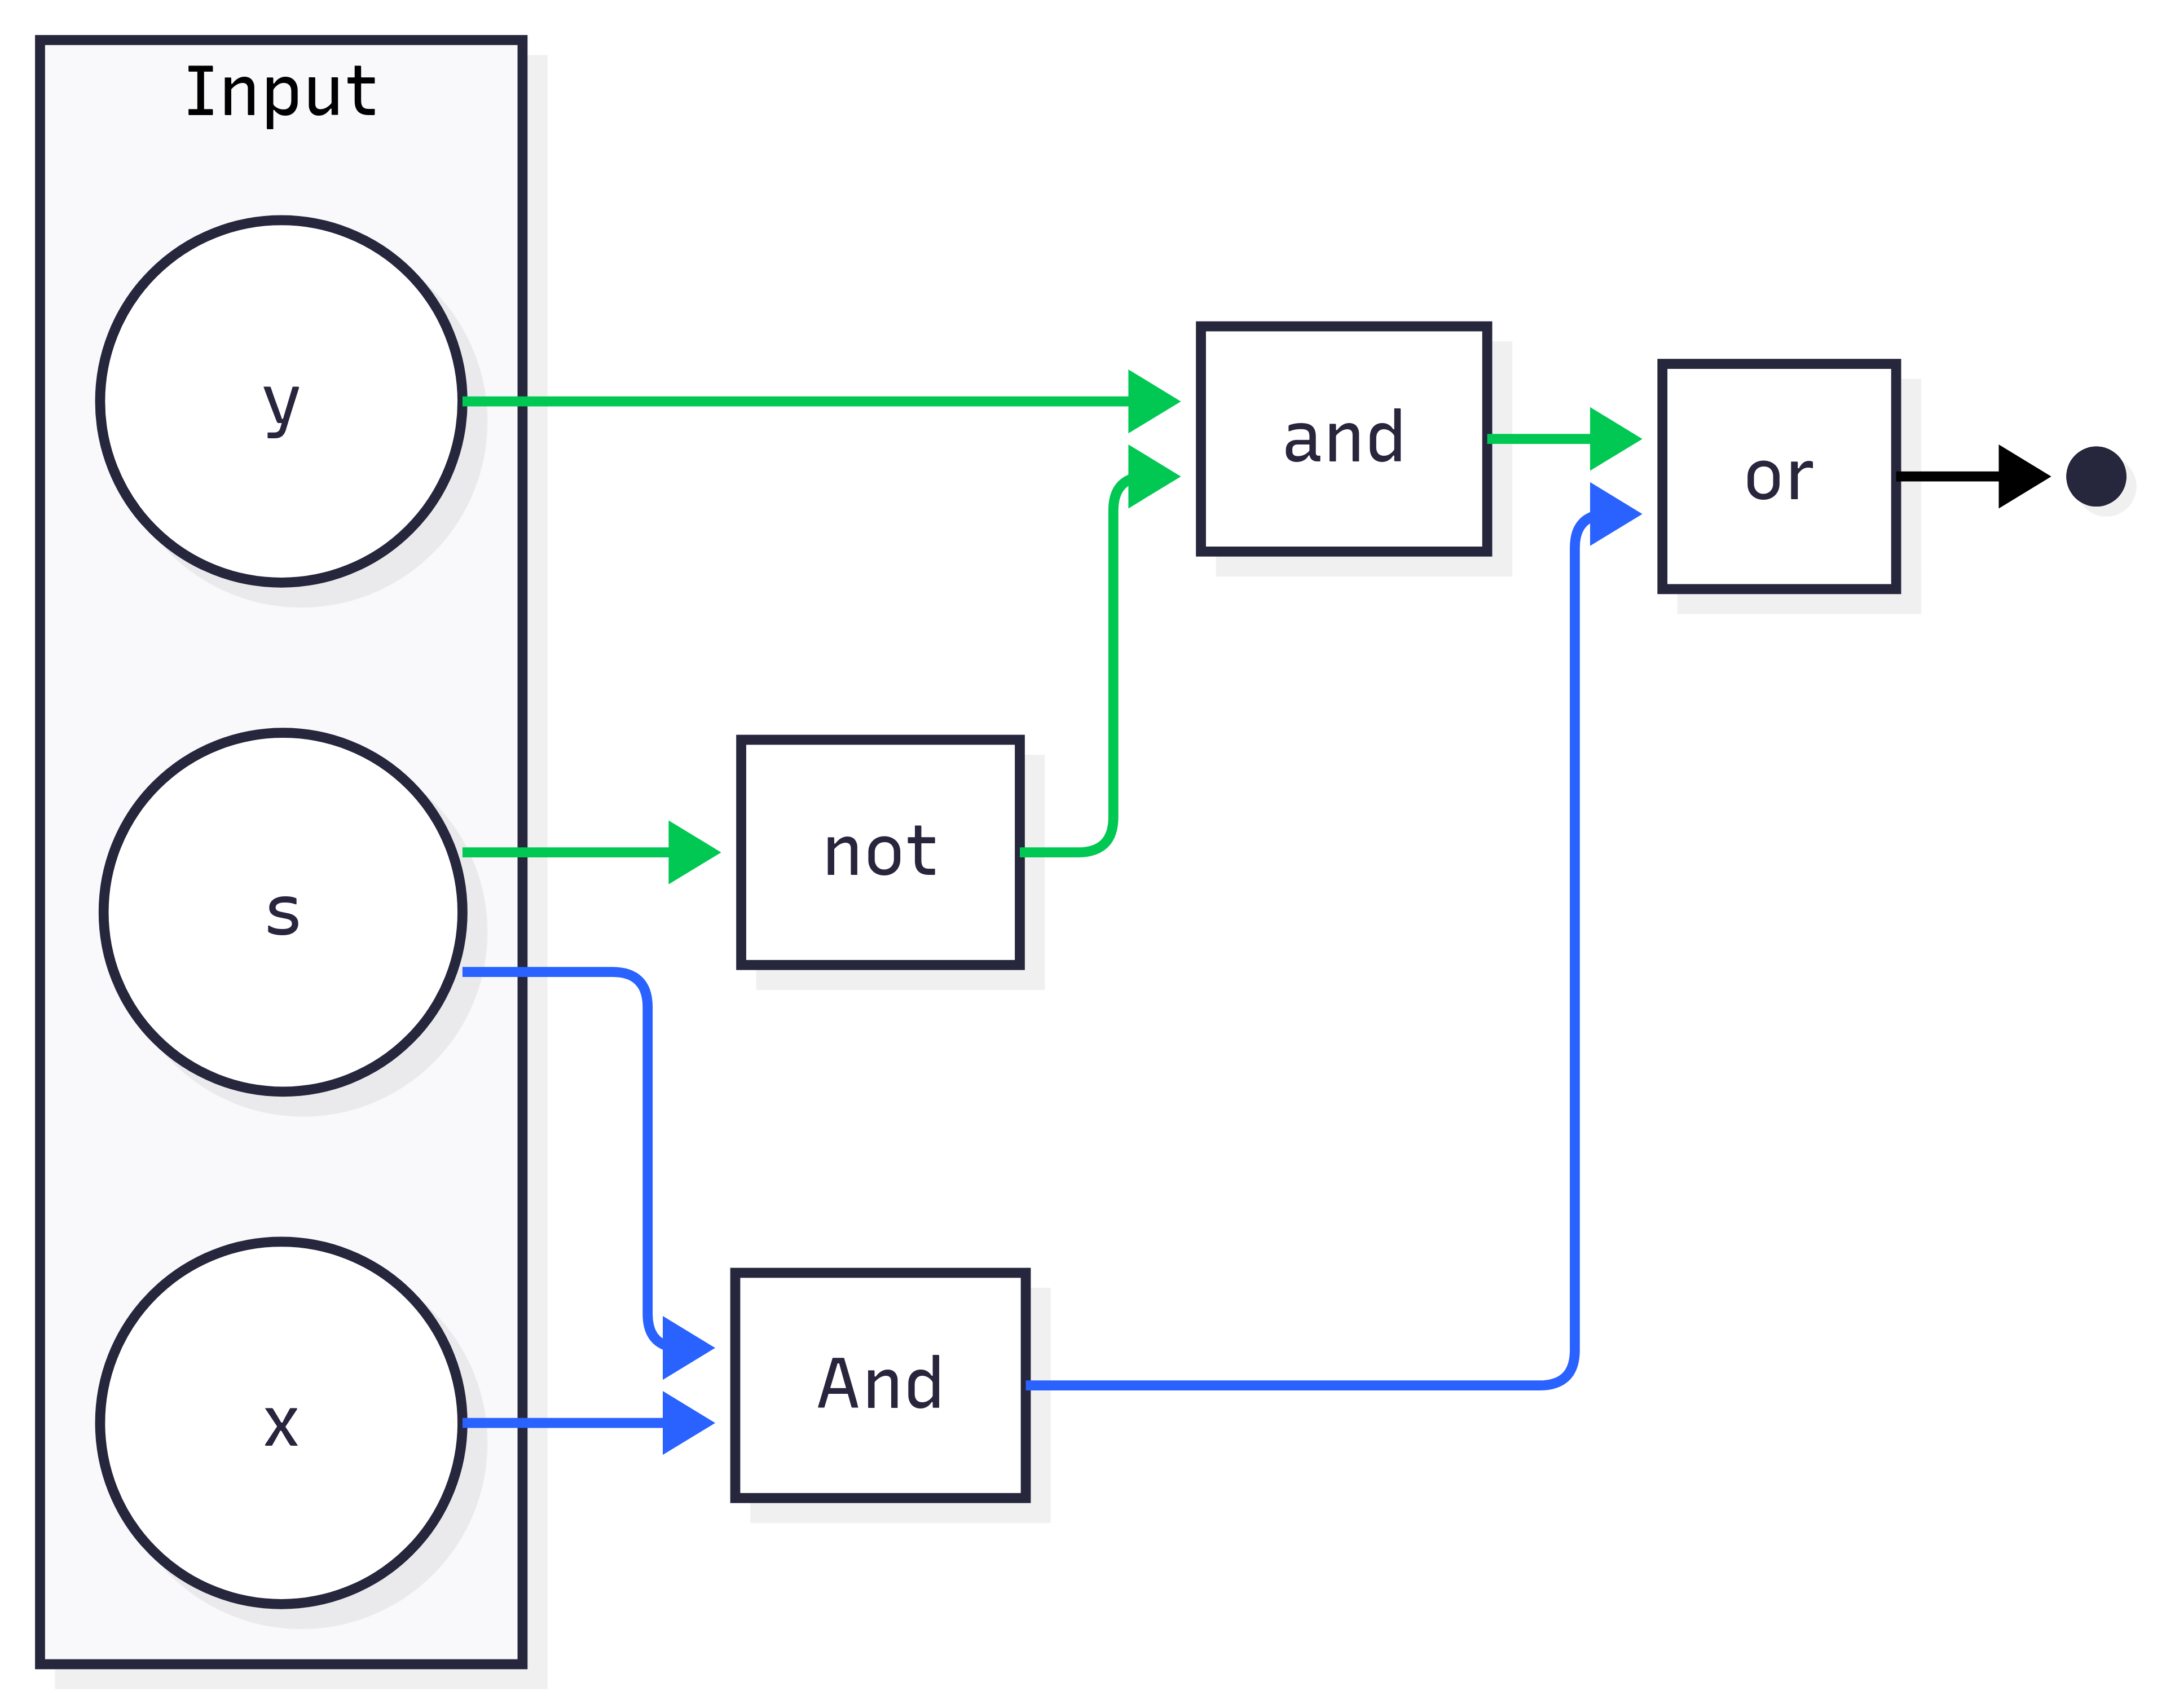
\includegraphics[width=0.3\textwidth]{assets/hazard_circuit.png}}
    \subfloat[Hazard free multiplexer]{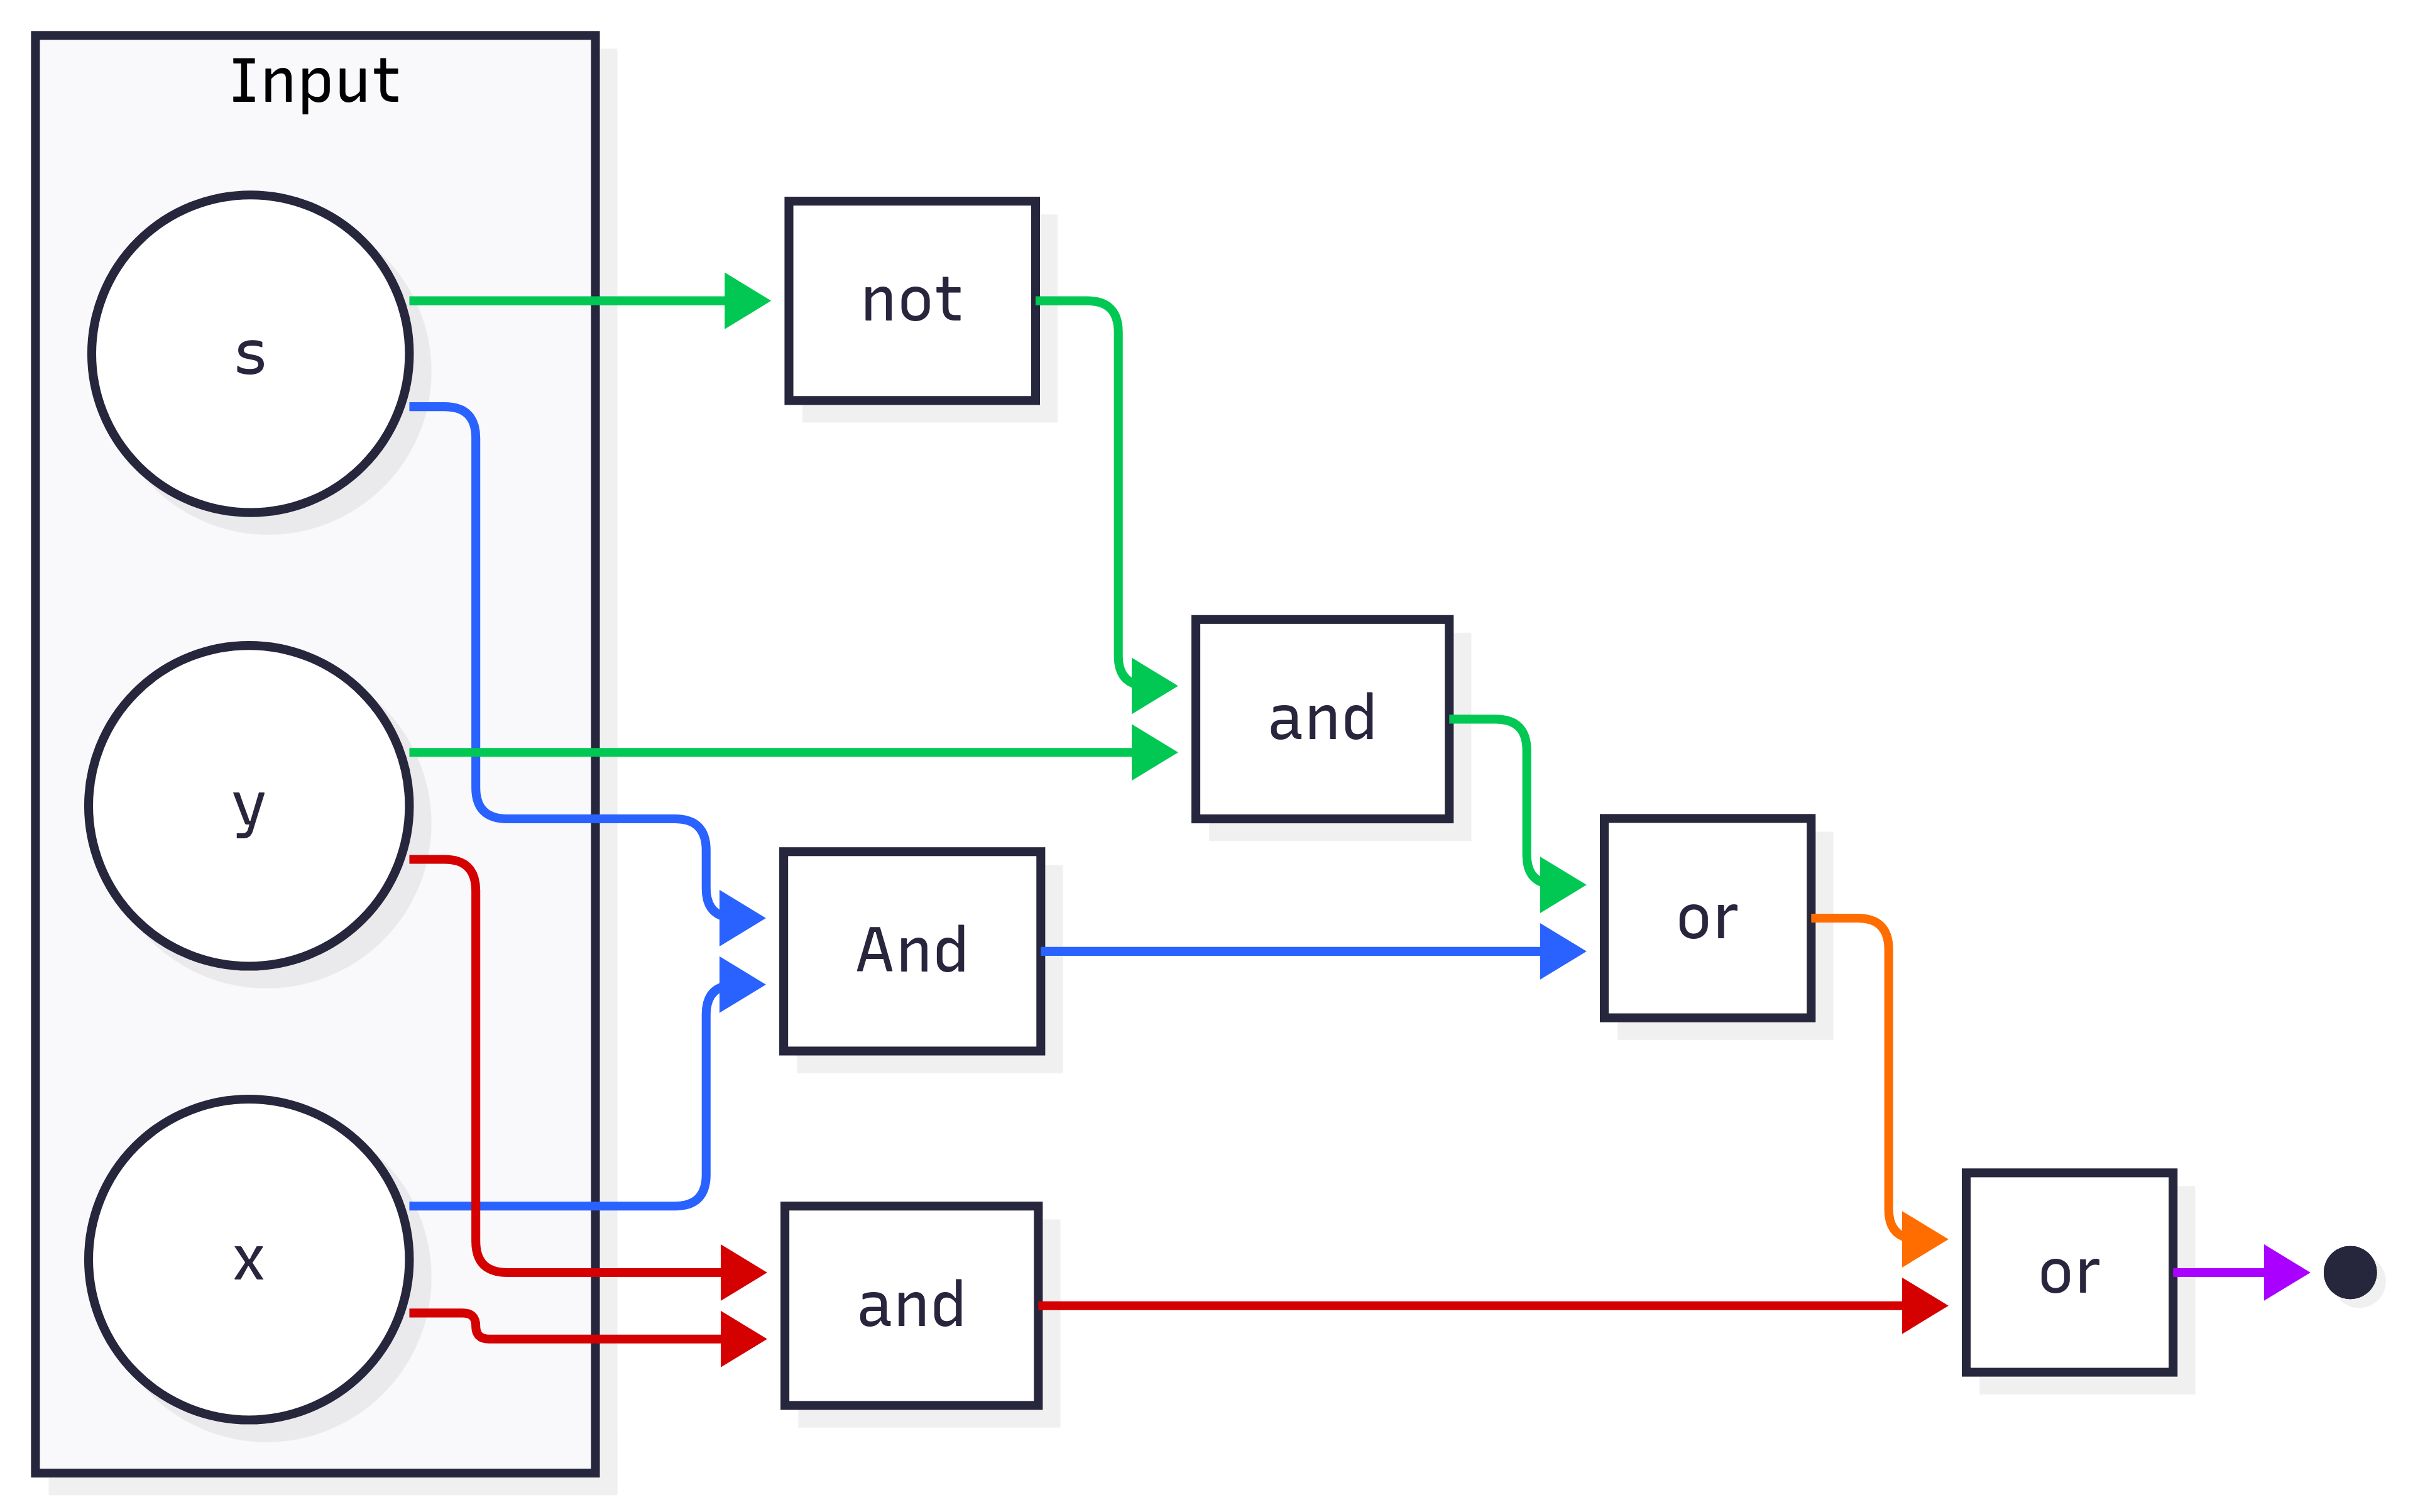
\includegraphics[width=0.3\textwidth]{assets/hazard-free-circuit.png}}
    \caption{Hazard circuit and hazard-free circuit. Figure by \cite{ikenmeyer_ComplexityHazardfreeCircuits_2019}}\label{fig:hazard-example}
\end{figure}

\begin{definitionbox}{K-bit Hazard \cite{ikenmeyer_ComplexityHazardfreeCircuits_2019}}{k-bit-haz}
    For $k \in \mathbb{N}$ a circuit $C: \mathbb{T}^n \to \mathbb{T}$ has a \textit{k-bit hazard} at $x \in \mathbb{T}^n$
    $\iff$ $C$ has a hazard at $x$ and $\bot$ appears at most $k$ times.
\end{definitionbox}
%
%
%
